% vim: set tw=78 tabstop=4 shiftwidth=4 aw ai:
\documentclass{beamer}

\usepackage[utf8]{inputenc}    % diacritice
\usepackage[english]{babel}
\usepackage{color}      % highlight
\usepackage{alltt}      % highlight
\usepackage{graphicx}
\graphicspath{{img/}}
\usepackage{tikz}
\usetikzlibrary{arrows.meta,positioning,calc}

% Code listings
\usepackage{listings}
\lstset{basicstyle=\ttfamily\small,columns=fullflexible,breaklines=true}

\usepackage{hyperref}      % folosiți \url{http://...}
% sau \href{http://...}{Nume Link}
\usepackage{verbatim}

\mode<presentation>
{%
  \usetheme{Madrid}
  \usecolortheme{dolphin}
}

% Light, modern-ish blue palette
\definecolor{PrismBlue}{RGB}{0,114,188}
\setbeamercolor{structure}{fg=PrismBlue}
\setbeamercolor{frametitle}{bg=PrismBlue!10,fg=PrismBlue!90!black}
\setbeamercolor{block title}{bg=PrismBlue!15,fg=PrismBlue!90!black}
\setbeamercolor{block body}{bg=PrismBlue!3,fg=black}
\setbeamercolor{author in head/foot}{bg=PrismBlue!90,fg=white}
\setbeamercolor{title in head/foot}{bg=PrismBlue!80,fg=white}
\setbeamercolor{upper separation line foot}{bg=PrismBlue!40}
\setbeamercolor{lower separation line foot}{bg=PrismBlue!40}

% Încărcăm simbolurilor Unicode românești în titlu și primele pagini
% (Removed \PreloadUnicodePage: not available with standard utf8 inputenc)

% Arătăm numărul frame-ului
\newcommand{\frameofframes}{/}
\newcommand{\setframeofframes}[1]{\renewcommand{\frameofframes}{#1}}

\setframeofframes{of}
\makeatletter
\setbeamertemplate{footline}
{%
  \begin{beamercolorbox}[colsep=1.5pt]{upper separation line foot}
  \end{beamercolorbox}
  \begin{beamercolorbox}[ht=2.5ex,dp=1.125ex,%
    leftskip=.3cm,rightskip=.3cm plus1fil]{title in head/foot}%
    \leavevmode{\usebeamerfont{institute in head/foot}\insertshortinstitute}%
    \hfill%
    {\usebeamerfont{title in head/foot}\insertshorttitle}%
    \hfill%
    {\usebeamerfont{frame number}\usebeamercolor[fg]{frame number}\insertframenumber~\frameofframes~\inserttotalframenumber}
  \end{beamercolorbox}%
  \begin{beamercolorbox}[colsep=1.5pt]{lower separation line foot}
  \end{beamercolorbox}
}
\makeatother

\setbeamertemplate{navigation symbols}{}%remove navigation symbols

% 3 logos (bottom-right) on slides after the title slide
\newcommand{\CornerLogos}{%
  \raisebox{-0.1cm}{\includegraphics[height=0.55cm]{logo-oficial-enupb_2.jpg}}\hspace{0.15cm}%
  \raisebox{-0.1cm}{\includegraphics[height=0.55cm]{images.jpg}}\hspace{0.15cm}%
  \raisebox{-0.1cm}{\includegraphics[height=0.55cm]{images.png}}%
}
\logo{\CornerLogos}

\title[Tickling x86\_64]{Tickling x86\_64: Detecting Emulator Inaccuracies Through CPU Instruction Forensics}
\subtitle{}
\author[Lafosse Louis]{\textbf{Lafosse Louis}\\
\scriptsize\texttt{louis.lafosse@stud.acs.upb.ro}\\
\textbf{Scientific Advisor: Adrian Razvan DEACONESCU}}
\date{February 1, 2026}

\begin{document}

% Slide-urile cu mai multe părți sunt marcate cu textul (cont.)
\setbeamertemplate{frametitle continuation}[from second]

\begingroup
\setbeamertemplate{logo}{}
\begin{frame}[plain]
  \vspace{0.2cm}
  \begin{columns}[T,onlytextwidth]

    \begin{column}{0.34\textwidth}
      \centering
      \includegraphics[height=1.2cm]{logo-oficial-enupb_2.jpg}\\[-0.2em]
      \scriptsize University POLITEHNICA of Bucharest
    \end{column}
    \begin{column}{0.33\textwidth}
      \centering
      \includegraphics[height=1.2cm]{images.jpg}\\[-0.2em]
      \scriptsize Faculty of Automatic Control and Computers
    \end{column}
    \begin{column}{0.33\textwidth}
      \centering
      \includegraphics[height=1.2cm]{images.png}\\[-0.2em]
      \scriptsize Computer Science and Engineering Department
    \end{column}
  \end{columns}

  \vspace{0.6cm}
  \titlepage
\end{frame}
\endgroup

\section{Project}
\begin{frame}{General project description}
  \begin{itemize}
    \item Goal: test how faithfully x86-64 CPU emulators match \textbf{native hardware} on subtle / security-critical behavior
    \item Scope: \textbf{8 targets} (Native, Blink, QEMU TCG, Box64, Icicle, Unicorn, MWEMU, KUBERA)
    \item Approach: small, focused micro-tests for edge cases + automated result parsing/formatting
    \item Why: emulator mismatches cause \textbf{false negatives} in security testing + enable \textbf{anti-emulation / fingerprinting / sandbox escaping} (CVE-2021-44078)
  \end{itemize}
\end{frame}

\section{Background}
\begin{frame}{Background and concepts}
  \begin{itemize}
    \item Emulation use cases: cross-arch execution, malware analysis sandboxes, binary translation, breaking obfuscation's
    \vspace{0.4em}
    \item Test focus (examples):
      \begin{itemize}
        \item x87 FPU \textbf{stack overflow} detection (SF/IE/C1 bits in status word)
        \item \textbf{LAHF} correctness (Load AH from FLAGS/RFLAGS registers)
        \item \textbf{RDTSCP} (Read Time-Stamp Counter and Processor ID)
      \end{itemize}
  \end{itemize}
\end{frame}

\begin{frame}{State of the Art: Problems \& Opportunities}
  \textbf{Current State:} 8+ emulators (Blink, QEMU, Unicorn, Box64, etc.) \\
  \textit{Tested for functionality, not security-relevant edge cases}
  
  \vspace{1em}
  
  \begin{columns}[T]
    \begin{column}{0.5\textwidth}
      \textcolor{red}{\textbf{Problems:}}
      \begin{itemize}
        \item Inconsistent edge-case behavior
        \item Security tool blind spots
        \item No systematic testing
      \end{itemize}
    \end{column}
    
    \begin{column}{0.5\textwidth}
      \textcolor{green!60!black}{\textbf{Opportunities:}}
      \begin{itemize}
        \item First systematic edge-case suite
        \item Security-focused testing
        \item Vulnerability discovery
        \item Emulator selection guide
      \end{itemize}
    \end{column}
  \end{columns}

\end{frame}

\section{Overview}
\begin{frame}{Project overview: architecture and objectives}
  \begin{itemize}
    \item Objectives:
      \begin{itemize}
        \item detect missing edge-case behavior (exceptions/flags)
        \item compare emulators side-by-side on identical tests
        \item extract \textbf{fingerprints} (behaviors that uniquely identify an emulator)
      \end{itemize}
    \item Architecture (high-level):
      \begin{itemize}
        \item tests generate small C/asm programs \textrightarrow compile \textrightarrow run under each emulator
        \item capture stdout/stderr \textrightarrow parse into structured results \textrightarrow report matrix
        \item special-case runners (e.g., Box64 PTY, Icicle JIT config, MWEMU panic handling)
      \end{itemize}
  \end{itemize}
\end{frame}

\section{Status}
\begin{frame}{Status so far (1/2): x87 FPU overflow}
  \begin{itemize}
    \item Expected on native hardware: status \textbf{\texttt{0x3a41}} (IE=1, SF=1, C1=1, TOP=7)
    \item Observed differences:
      \begin{itemize}
        \item Native + Blink: \textbf{correct} overflow detection
        \item QEMU / Box64 / Unicorn: \textbf{missing} overflow flags (e.g., \texttt{0x3800})
        \item Icicle: no FPU (\texttt{0x0000}); MWEMU panics; KUBERA unsupported
      \end{itemize}
  \end{itemize}
\end{frame}


\begin{frame}{Status so far (1/2): x87 FPU overflow explanation}
  \vspace{-0.2cm}
  \begin{columns}[T,onlytextwidth]
    \begin{column}{0.56\textwidth}
      \centering
      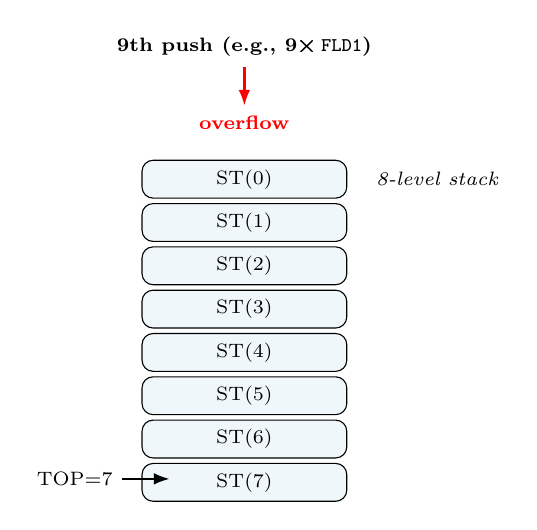
\begin{tikzpicture}[font=\scriptsize, every node/.style={align=center}]
        % Stack boxes (top to bottom)
        \foreach \i in {0,...,7} {
          \pgfmathtruncatemacro{\y}{7-\i}
          \node[draw,rounded corners,minimum width=2.6cm,minimum height=0.45cm,fill=PrismBlue!6]
            (st\i) at (0,0.55*\y) {ST(\i)};
        }

        % Indicate 8th is full
        \node[anchor=west] at (1.55,0.55*7) {\textit{8-level stack}};

        % "9th push" arrow
        \draw[-{Latex[length=2mm]},thick,red] (0,0.55*9.6) -- (0,0.55*8.7)
          node[pos=0,above,black] {\textbf{9th push (e.g., 9\texttimes\,\texttt{FLD1})}}
          node[pos=1,below,red] {\textbf{overflow}};

        % TOP pointer example
        \draw[-{Latex[length=2mm]},thick] (-1.55,0.55*0.08) -- (-0.95,0.55*0.08);
        \node[anchor=east] at (-1.55,0.55*0.08) {TOP=7};
      \end{tikzpicture}

      \vspace{0.3em}
      \scriptsize
      Example test:\;\texttt{finit; fld1 (\texttimes 9); fnstsw ax}
    \end{column}

    \begin{column}{0.44\textwidth}
      \begin{block}{FPU status word bits set on overflow}
        \scriptsize
        \begin{tabular}{@{}ll@{}}
          \textbf{IE} (bit 0)  & Invalid Operation = 1 \\
          \textbf{SF} (bit 6)  & Stack Fault = 1 \\
          \textbf{C1} (bit 9)  & Overflow direction = 1 \\
          \textbf{TOP} (11--13)& Updated stack top (e.g., 7) \\
        \end{tabular}

        \vspace{0.4em}
        Expected (native): \textbf{\texttt{0x3a41}}
      \end{block}

      
    \end{column}
  \end{columns}
\end{frame}

\begin{frame}{Status so far (2/2): fingerprints \& security}
  \begin{itemize}
    \item \textbf{LAHF}: Blink sets AF incorrectly (\texttt{0x0b} vs expected \texttt{0x03}) \textrightarrow reliable fingerprint
    \item \textbf{RDTSCP (TSC\_AUX)}: Blink returns \texttt{0x00} consistently \textrightarrow reliable fingerprint
    \item \textbf{Security finding}: Unicorn Engine \texttt{uc\_context\_restore()} context-type mismatch can trigger a heap buffer overflow (responsible disclosure in progress)
  \end{itemize}
\end{frame}

\section{Plan}
\begin{frame}{Plan for next semester}
  \begin{itemize}
    \item Expand test coverage:
      \begin{itemize}
        \item memory ordering / atomics (LOCK, fences)
        \item segment register edge cases (FS/GS base)
        \item CPUID leaves / topology, timer precision
        \item AVX/AVX2 (optionally AVX-512 if supported)
      \end{itemize}
    \item Rework / Optimisation of Sandsifter x86 fuzzer
    \item Upstream work:
      \begin{itemize}
        \item QEMU-TCG, Box64, Icicle, Mwemu missing x87 overflow detection (where feasible)
        \item Blink LAHF, RDTSCP detection patch
        \item \textbf{Unicorn}: coordinated upstream disclosure + patch for \texttt{uc\_context\_restore()} validation
      \end{itemize}
  \end{itemize}
\end{frame}

\section{Thanks}
\begin{frame}[plain]
  % subtle background accent
  
\begin{tikzpicture}[remember picture,overlay]
    \fill[PrismBlue!6] (current page.south west) rectangle ([yshift=2.2cm]current page.south east);
    \fill[PrismBlue!10] (current page.north west) rectangle ([yshift=-1.2cm]current page.north east);
  \end{tikzpicture}

  \vspace{1.3cm}
  \begin{center}
    {\color{PrismBlue!90!black}\fontsize{34}{38}\selectfont\textbf{Thank you}}\\[0.35em]
    {\Large\color{PrismBlue!80!black}Questions?}\\[1.1em]

    \vspace{0.8em}
    {\small\color{PrismBlue!70!black}
    \url{https://github.com/louislafosse/research-polytechnic}}
  \end{center}

  \vfill
  \begin{center}
    \CornerLogos
  \end{center}
\end{frame}

\end{document}
